
\section{Introduction to discrete random-time processes}
\textbf{Parametric random process}
\[
x[n]=f(a,n)
\]
Where \(a\) is a vector of random parameters,example:
\[
x[n]=A\cos(2\pi F_0 n+\theta_0)
\]
Generally \(A\) is modelled as a Rayleigh random variable while the phase is typically modelled as a r.v uniformally distributed in \([-\pi,+\pi)\)
\[
A\in[\mathcal{R(\sigma^2)}] \text{ and } f_A(a)=\frac{a}{\sigma^2_A}e^{-\frac{a^2}{2\sigma^2_A}}u(a),\hspace{0.25em}E\{A^2\}=2\sigma^2_A
\]
\textit{Important}, the two variables are indipendet so the probability is the joint one.
\begin{figure}[H]
    \centering
    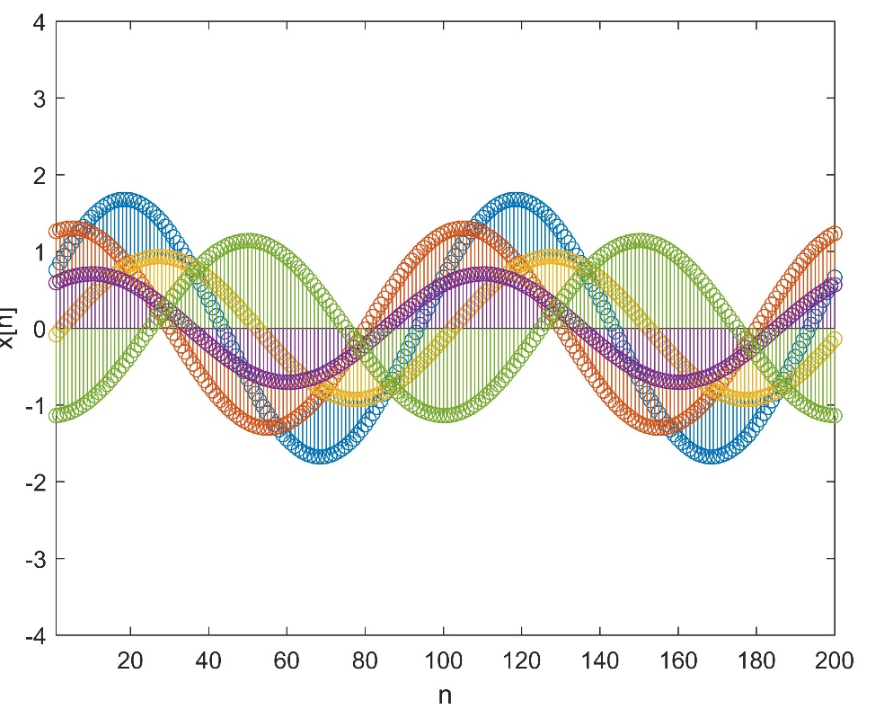
\includegraphics[width=0.5\linewidth]{Image/chap 1/4.example.png}
   
\end{figure}
\noindent More in general a parametric process is fully characterized by the function \(f(\mathbf{a},n)\) and by the joint pdf of the random parameters.\\
È la stessa cagata che fai con il rumore, ha trovato semplicemente dei modelli matematici per quei dati parametri.
\subsection{Characterization of a discrete-time random process}
\begin{itemize}
    \item \textbf{Cumulative distribution function (cdf)}
    \[
    P_x(x_1,x_2,...,x_N;n_1,n_2,...n_N) = Pr\{x[n_1]\leq x_1,x[n_2]\leq x_2,...,x[n_N]\leq x_N\}
    \]
    Reminder: ho preso un set di \(N\) di random variables sampled from \(x[n]\)
    \item \textbf{Probability density funcntion(pdf)}
    \[
    p_X(x_1,x_2,...,x_N;n_1,n_2,...n_N) =\frac{\partial^N P_X(x_1,x_2,...,x_N;n_1,n_2,...n_N)}{\partial x_1 \partial x_2...\partial x_N}
    \]
\end{itemize}
Tutta sta manfrina per dire che alla fine sta roba non riesci quasi mai a farla quindi usi:
\textbf{statistical indices}.
\subsubsection{First order statistics}
They concern one single variable so they require knowledge of only the first order pdf:
\begin{itemize}
    \item \textbf{Moment of order k}:\[
    E\{x^k[n]\}=\int_{-\infty}^{+\infty} x^kp_X(x;N) dx
    \]
    \item \textbf{Mean}
    \[
    \eta_X[n] =E\{x[n]\} =\int_{-\infty}^{+\infty}xp(x;n) dx
    \]
    \item \textbf{Statistical power}
    \[
    P_X[n]=E\{x^2[n]\}=\int_{-\infty}^{+\infty} x^2p(x;n)dx
    \]
    \item \textbf{Variance}
    \[
    \sigma^2_X[n]=E\{(x[n]-\eta_X[n])^2\} =\int_{-\infty}^{+\infty}(x-\eta_X[n])^2 p_X(x;n)dx=P_X[n]-\eta_X^2[n]
    \]
\end{itemize}
\subsubsection{Second order statistics}
They concern two variable extracted from the process so they require knowledge of the second order of the pdf.
\begin{itemize}
    \item \textbf{Autocorrelation function (ACF)}
     \[
     R_X[n_1, n_2] \triangleq E\{ x[n_1] x[n_2] \} \triangleq 
     \int_{-\infty}^{+\infty} \int_{-\infty}^{+\infty} x_1 x_2\, p_X(x_1, x_2; n_1, n_2) \, dx_1 dx_2
     \]
     \item \textbf{Covariance function}:
     
     \[
C_X[n_1, n_2] \triangleq E\left\{ (x[n_1] - \eta_X[n_1])(x[n_2] - \eta_X[n_2]) \right\} = R_X[n_1, n_2] - \eta_X[n_1] \eta_X[n_2]
\]
\item Some conditions \begin{itemize}
    \item \textit{Orthogonal}: \[
    R_X[n_1,n_2]=E\{x[n_1]x[n_2]\}=0
    \]
    \item \textit{Uncorrelated}
    \[C_X(n_1,n_2)=0\rightarrow R_X[n_1,n_2=\eta_X[n_1]\eta_X[n_2]]\]
\end{itemize}
\item Note:
\[
P_X[n] = R_X[n, n], \qquad \sigma_X^2[n] = C_X[n, n]
\]


\end{itemize}
\subsection{Stationariety}
\subsubsection{Strict sense}
A discrete random process \(x[n]\) is said to be stationary in strict sense if its joint pdf of any order is invariant to any shift:
\[
p_X(x_1, x_2, \ldots, x_N; n_1, n_2, \ldots, n_N) = p_X(x_1, x_2, \ldots, x_N; n_1 - L, n_2 - L, \ldots, n_N - L)
\]
\[
\forall N \in \mathbb{N},\;\; \forall \mathcal{S}_N = \{ n_1, \ldots, n_N \},\;\; \forall L \in \mathbb{Z}
\]
The strict sense mean that \(x[n]\) and its shifted version are statistically equivalent, this does not imply that \(x[n]=x[n-L]\).
\subsubsection{Wide sense}
A discrete random process \(x[n]\) is said to be wide-sense stationary if its mean is constant and its ACF is only in function of the spacing between the sampled random variables(\(lag\))
\begin{itemize}
    \item \[\eta_X[n]=\eta_X\]
    \item \[R_X[n_1,n_2]=R_X[0,n_2-n_1]=R_X[m]\]
    \begin{itemize}
        \item \[
C_X[n_1, n_2] \equiv C_X[0, n_2 - n_1] \equiv C_X[m]
\]
\item 
\[
\sigma_X^2[n] = C_X[n, n] \equiv C_X[0] \triangleq \sigma_X^2
\]
\item 
\[
P_X[n] = R_X[n, n] \equiv R_X[0] \triangleq P_X = \sigma_X^2 + \eta_X^2
\]
    \end{itemize}
\end{itemize}
REMEMBER: strict implies wide, while the reverse is not true. Unless the process is gaussian.
\subsection{Proprierties of the ACF}
\begin{enumerate}

    \item \textbf{Simmetry}: \[
R_X[m] = E\left\{ x[n]\, x[n + m] \right\}
        = E\left\{ x[n - m]\, x[n] \right\}
        = E\left\{ x[n]\, x[n - m] \right\}
        = R_X[-m]
\]
    The same property for :
    \[
    C_X[m]=C_X[-m]
    \]
    \item  The ACF has is maximum value in 0, grazie al cazzo sono due function allineate in quanto sono la stessa funzione il massimo sarà quando sono sovrapposte :
    \[
    R_X[0]\geq |R_X[m]|,\hspace{0.25em}\forall \in\mathbb{Z}
    \]
  \[
    C_X[0]\geq|C_X[m]|,\hspace{0.25em}\forall \in \mathbb{Z}
    \]
    \item If \(x[n]\) is a w.s.s discrete-time \textit{complex-valued} process, its ACF satisfies the HERMITIAN SIMMETRY property:
    \[
R_X[m] \triangleq E\left\{ x[n] x^*[n + m] \right\}
= E\left\{ x[n - m] x^*[n] \right\}
= \left( E\left\{ x[n] x^*[n - m] \right\} \right)^*
= R_X^*[-m]
\]
    \item If \(x[n]\) contains a periodic component with period \(N_0\), then the ACF and the correlation function contain a periodic component of the same period \(N_0\):
    \[
R_X[m] = E\left\{ x[n] x[n + m] \right\}
= E\left\{ x[n] x[n + m - N_0] \right\}
= R_X[m - N_0]
\]
\item If the ACF of a stationary process does not contain periodic components, then :

\[
\lim_{m \to \infty} R_X[m]
= \lim_{m \to \infty} \left[ C_X[m] + \eta_X^2 \right]
= \lim_{m \to \infty} C_X[m] + \eta_X^2
= \eta_X^2
\]
This because, if the process does not contain periodic omponents, when the lag \(m\) increases the two random variables \(x[n]\) and \(x[n+m]\) tend to be uncorrelated.
\end{enumerate}
\subsection{Discrete processes and random vectors}
\begin{itemize}
    \item Let \texttt{x} be a random vector consisting of \(N\) random variables sampled froma a discrete-time random process \(x[n]\):
    \[
    \mathbf{x}=[x[0]\hspace{0.35em}x[0]\hspace{0.35em}\dots\hspace{0.35em}x[N-1]]^T \in\mathbb{R}^N   \]
    \item The mean valure is defined as:
    \[
\mathbf{\eta}_x \triangleq E\{\mathbf{x}\} = \left[ E\{x[0]\}\; E\{x[1]\}\; \cdots\; E\{x[N-1]\} \right]^T = \left[ \eta_x[0]\; \eta_x[1]\; \cdots\; \eta_x[N-1] \right]^T
\]
\item For a w.s.s random process, the mean vector has all its components equal to the same value:
\[
\left[ \eta_x \right]_{n+1} = E\{x[n]\} = \eta_x, \quad n = 0, 1, \ldots, N-1 \quad \Rightarrow \quad \mathbf{\eta}_x = \eta_x \left[ 1 \;\; 1 \;\; \cdots \;\; 1 \right]^T = \eta_x \mathbf{1}
\]
\item The \textbf{correlation matrix} is defined as:
\[
\mathbf{R}_x \triangleq E\{\mathbf{xx}^T\}\in\mathbb{R}^{N\times N}
\]
\item \(\mathbf{R}_x\) is symmetric and positive semidefinite:
\[
\mathbf{R}_x = E\{ \mathbf{x} \mathbf{x}^T \} = E\left\{ \left( \mathbf{x} \mathbf{x}^T \right)^T \right\} = \left( E\{ \mathbf{x} \mathbf{x}^T \} \right)^T = \mathbf{R}_x^T
\]

\[
\text{EVD: } \quad \mathbf{R}_x = \mathbf{U} \mathbf{\Lambda} \mathbf{U}^T, \quad \lambda_k = [\mathbf{\Lambda}]_k \geq 0 \quad \forall k
\]

\[
\text{Eigenvalue-Eigenvector Decomposition (EVD)}
\]
\item The correlation matrix of \textbf{x} is completely specified by the correlation function of the process \(x[n]\):
\[
\left[ \mathbf{R}_x \right]_{i+1,\,j+1} = E\left\{ x[i]\,x[j] \right\} = R_x[i,\,j], \quad i, j = 0, 1, \ldots, N-1
\]
\item If \(x[n]\) is a w.s.s, \(\mathbf{R}_x\) is not only symmetric, but it is also a \textbf{Toeplix} matrix, i.e.:
\[
\left[ \mathbf{R}_x \right]_{i+1,\,j+1} = E\left\{ x[i]\,x[j] \right\} = R_x[i,\,j] = R_x[j-i],\quad i, j = 0, 1, \ldots, N-1
\]

\[
\mathbf{R}_x =
\begin{bmatrix}
R_x[0] & R_x[1] & \cdots & R_x[N-1] \\
R_x[-1] & R_x[0] & \cdots & R_x[1] \\
\vdots & \vdots & \ddots & \vdots \\
R_x[-(N-1)] & \cdots & R_x[-1] & R_x[0]
\end{bmatrix}
= \mathbf{R}_x^T
\]
A \textbf{Toeplitz} matrix has a structure with some implications for the calculation of its inverse.
\item The \textbf{covariance matrix} of \textbf{x} is defined as:
\[
\mathbf{C}_x \triangleq E\left\{ (\mathbf{x} - \mathbf{\eta}_x)(\mathbf{x} - \mathbf{\eta}_x)^T \right\} = \mathbf{R}_x - \mathbf{\eta}_x \mathbf{\eta}_x^T \in \mathbb{R}^{N \times N}
\]
\(\mathbf{C}_x\) is symmetric and positive semidefinite.
\item The covariance matrix of \textbf{x} is completely specified by the covariance function of \(x[n]\):
\[
\left[ \mathbf{C}_x \right]_{i+1,\,j+1} = E\left\{ \left(x[i] - \eta_x[i]\right)\left(x[j] - \eta_x[j]\right) \right\} = C_x[i,\,j],\quad i, j = 0, 1, \ldots, N-1
\]

\[
\text{Se } x[n] \text{ è w.s.s.,} \;\; \mathbf{C}_x \text{ è anche una matrice di Toeplitz, i.e.}
\]

\[
\left[ \mathbf{C}_x \right]_{i+1,\,j+1} = C_x[j-i] \implies
\mathbf{C}_x =
\begin{bmatrix}
C_x[0] & C_x[1] & \cdots & C_x[N-1] \\
C_x[-1] & C_x[0] & \cdots & C_x[1] \\
\vdots & \vdots & \ddots & \vdots \\
C_x[-(N-1)] & \cdots & C_x[-1] & C_x[0]
\end{bmatrix}
= \mathbf{C}_x^T
\]
\end{itemize}
\subsection{Gaussin discrete random processes}
\begin{itemize}
    \item A discrete-time random process \(x[n]\) is said to be \textit{Gaussian} if every set of \(N\) random variables \(\{x[n_1],x[n_2],\cdots,x[n_N]\}\) are jointly Gaussian distributed for every N-tuple \(\{n_1,\cdots,n_2\}\).
    \item Alternatively, \(x[n]\) is said to be \textit{Gaussian} if the vector of random variables:
    \[
\mathbf{x} = \left[ x[n_0]\;\; x[n_0+1]\;\; \cdots\;\; x[n_0+N-1] \right]^T,\quad \forall n_0,\, \forall N
\]
\(
\text{has a Gaussian pdf with mean value } \eta_x \text{ and covariance matrix } \mathbf{C}_x \text{:}
\)
\[
f_x(\mathbf{x}) = \frac{1}{\sqrt{(2\pi)^N|\mathbf{C}_x|}} \exp\left[ -\frac{1}{2} (\mathbf{x} - \eta_x)^T \mathbf{C}_x^{-1} (\mathbf{x} - \eta_x) \right]
\]

\[
\mathbf{x} \sim \mathcal{N}\left( \eta_x,\; \mathbf{C}_x \right)
\]

\item \texttt{IMPORTANT}: The pdf of any order \(N\) of a Gaussian vector \textbf{x} is fully characaterized by the knowledge of the mean value vector \(\eta_X\) and the covariance matrix \(C_X\)
\item \texttt{IMPORTANT}: The gaussianity property is invariant under affine trasformations.

\[
\mathbf{x} \sim \mathcal{N}(\mathbf{\eta}_x,\, \mathbf{C}_x)
\quad \Longrightarrow \quad
\mathbf{y} = \mathbf{A}\mathbf{x} + \mathbf{b} \sim \mathcal{N}(\mathbf{A}\mathbf{\eta}_x + \mathbf{b},\, \mathbf{A}\mathbf{C}_x\mathbf{A}^T)
\]

\[
\mathbf{\eta}_y = E\{\mathbf{y}\} = E\{\mathbf{A}\mathbf{x} + \mathbf{b}\} = \mathbf{A}E\{\mathbf{x}\} + \mathbf{b} = \mathbf{A}\mathbf{\eta}_x + \mathbf{b}
\]

\[
\mathbf{C}_y = E\left\{ (\mathbf{y} - \mathbf{\eta}_y)(\mathbf{y} - \mathbf{\eta}_y)^T \right\}
= E\left\{ (\mathbf{A}\mathbf{x} - \mathbf{A}\mathbf{\eta}_x) (\mathbf{A}\mathbf{x} - \mathbf{A}\mathbf{\eta}_x)^T \right\}
\]

\[
= E\left\{ \mathbf{A}(\mathbf{x} - \mathbf{\eta}_x)(\mathbf{x} - \mathbf{\eta}_x)^T \mathbf{A}^T \right\}
= \mathbf{A} E\left\{ (\mathbf{x} - \mathbf{\eta}_x)(\mathbf{x} - \mathbf{\eta}_x)^T \right\} \mathbf{A}^T
= \mathbf{A}\mathbf{C}_x\mathbf{A}^T
\]
\item \texttt{IMPORTANT}: Every r-tuple of random variables taken from a Gaussian vector \textbf{x} of dimension \(N\) with \(r<N\) forms a Gaussian vector of dimension \(r\).  \\
In particular, each entry of a Gaussin random vectori is a Gaussian r.v.:
\[
\left[ \mathbf{x} \right]_k \sim \mathcal{N}\left( \left[ \mathbf{\eta}_x \right]_k,\, \left[ \mathbf{C}_x \right]_{k,k} \right)
\]
\item \texttt{IMPORTANT}: Every r-tuple of random variables taken from a Gaussian vector \textbf{x} conditioned to another \(k-\)tuple, also taken froma the same vector \textbf{x}, are (conditionally) Gaussian distributed.
\item If \(N\) jointly Gaussian random variables \(\{x[n]\}'\) are mutually uncorrelated, they are also mutually independent.
\newpage
\[
\text{If:} \quad c_{X_i, X_j} = \mathrm{cov}\{x[i], x[j]\} = 0 \quad \text{for} \quad i \neq j \implies \mathbf{C}_X =
\begin{bmatrix}
\sigma_{X_1}^2 & 0 & \cdots & 0 \\
0 & \sigma_{X_2}^2 & \cdots & 0 \\
\vdots & \vdots & \ddots & \vdots \\
0 & 0 & \cdots & \sigma_{X_N}^2
\end{bmatrix}
\, \] 
\[
\text{where} \quad \sigma_{X_i}^2 \triangleq \mathrm{var}\{x[i]\}
\]\[
\text{Then:} \quad
(\mathbf{x} - \boldsymbol{\eta}_X)^T \mathbf{C}_X^{-1} (\mathbf{x} - \boldsymbol{\eta}_X) =
\sum_{i=1}^N \frac{(x_i - \eta_{X_i})^2}{\sigma_{X_i}^2}
\quad \text{and} \quad
|\mathbf{C}_X| = \prod_{i=1}^N \sigma_{X_i}^2 
\]\[
\text{Hence:} \quad
f_X(\mathbf{x}) = \frac{1}{\sqrt{(2\pi)^N \prod_{i=1}^N \sigma_{X_i}^2}}
\exp\left[-\frac{1}{2} \sum_{i=1}^N \frac{(x_i - \eta_{X_i})^2}{\sigma_{X_i}^2}\right]
= \]\[\prod_{i=1}^N \frac{1}{\sqrt{2\pi \sigma_{X_i}^2}} \exp\left[
-\frac{(x_i - \eta_{X_i})^2}{2\sigma_{X_i}^2}
\right]
= \prod_{i=1}^N f_{X_i}(x_i)
\]
\end{itemize}
\subsection{Stationary discrete-time white process}
\begin{itemize}
    \item A zero-mean, stationary (at least in wide-sense), discrete-time random process \(x[n]\) is called a \textbf{white process}, or a white noise process, if the random variables sampled from it are pairwise uncorrelated.
    \item The mean value and ACF of a discrete-time white process can be expressed as:
    \[
    \eta_X=0
    \]
    \[
    R_X[m]=C_X[m]=\sigma^2_X\delta[m]=\begin{cases}
        \sigma^2_X, \hspace{0.25em} m=0\\
        0, \hspace{0.25em}m\neq0
    \end{cases}
   \]
   We say the process is \(\delta-\)correlated.
   A discrete-time white process need not to be Gaussian. The only requirement is that ist mean is zero and the sampled r.v.'s are uncorrelated.
   \item \texttt{IMPORTANT}: If the random variables \(\{x[n]\}\)'s have been obtained by sampling a white gaussian process, they are not only uncorrelated, but also independent.
\end{itemize}
In particular, if the process is w.s.s white gaussian process, the \(\{x[n]\}'s\) are \underline{independet and identically}\\ \underline{distributed(IID)}.
\[
\eta_{X_i} \triangleq E\{x[n]\} = \eta_X,\qquad \sigma_{X_i}^2 \triangleq \mathrm{var}\{x[i]\} = \sigma_X^2 \qquad \forall i
\]
(se $\mathbf{W}$ white $=0$)

\[
\Downarrow
\]
\[
\text{Per processo di variabili indipendenti:}\qquad
\boldsymbol{\eta}_X = \eta_X \mathbf{1},\qquad \mathbf{C}_X = \sigma_X^2 \mathbf{I} \text{ (matrice identità)}
\]
\[
\Downarrow
\]

\[
f_X(\mathbf{x}) = \prod_{i=1}^N f_{x_i}(x_i) = \prod_{i=1}^N \frac{1}{\sqrt{2\pi\sigma_X^2}}
\exp\left( -\frac{(x_i - \eta_X)^2}{2\sigma_X^2} \right)
\]
IMPORTANT EXAMPLE: Let \(v[n]\) of IID random variables with mean \(\eta\) and variance \(\sigma^2\). The ACF of \(v[n]\) is :
\[
R_V[n_1, n_2] = E\{ v[n_1] v[n_2] \} = 
\begin{cases}
    E\{v[n_1]\} E\{v[n_2]\} = \eta^2, & n_1 \neq n_2 \\
    E\{v^2[n_1]\} = \sigma^2 + \eta^2, & n_1 = n_2
\end{cases}
\]
The ACF can be rewritten as :
\[
R_V[n_1,n_2]=\sigma^2\delta[n_2-n_1]+\eta^2
\]
Since the mean is constant and the ACF is a function only of the difference \(m\), \(v[n]\) is a discrete-time random process.\\
If the mean is also \(=0\), \(v[n]\) is a w.s.s discrete time random process.
SERIES EXAMPLE PDF 2, start around slide 30(good exercise)
\subsection{Cross-correlation and cross-variance functions}
\begin{itemize}
    \item It is often necessary to deal with correlations(or covariances) between two or more random processes.
    \item To this purpose, the \textbf{cross-correlation function} between two discrete-time random processes, \(x[n]\) and \(y[n]\), can be defined as:
    \[
    R_{XY}[n_1,n_2]\triangleq E\{x[n_1]y[n_2]\}
    \]
    \item Similarly, the \textbf{cross-covariance function} is defined as:
    \[
    C_{XY}[n_1,n_2]\triangleq E\{(x[n_1]-\eta_X[n_2])(y[n_2]-\eta_Y[n_2])\}=R_{XY}[n_1,n_2]-\eta_X[n_1]\eta_Y[n_2]
    \]
    \item Two random processes, \(x[n]\) and \(y[n]\), are said to be orthogonal if their cross-correlation function is identical to zero.
    \item \(x[n]\) and \(y[n]\) are said to be uncorrelated if their cross-covariance function is zero.
    \item Two discrete random processes, \(x[n]\) and \(y[n]\), are said to be wide sense \textit{jointly stationary} if:
    \begin{enumerate}
        \item \(x[n]\) and \(y[n]\) are wide-sense stationary;
        \item The cross-correlation function is a function of only the lag \(m=n_2-n_1\)
        \[
        R_{XY}[n_1,n_2]=R_{XY}[0,n_2-n_1]\equiv R_{XY}[n_2-n_1]\equiv R_{XY}[m]
        \]
        \item If \(x[n]\) and \(y[n]\) are \textit{jointly stationary}, then the cross-correlation and the cross-covariance functions are functions only of the lag \(m=n_2-n_1\)
        \[
R_{XY}[n_2-n_1] \equiv R_{XY}[m] \triangleq E\{ x[n] y[n+m] \}
\]

\[
C_{XY}[n_2-n_1] \equiv C_{XY}[m] \triangleq E \left\{ (x[n] - \eta_X)(y[n+m] - \eta_Y) \right\} = R_{XY}[m] - \eta_X \eta_Y
\]
    \end{enumerate}
\end{itemize}
The cross-correlation and the cross-covariance fucntions have no special symmetry(they can even be one-sided).\\
The correlation between \(x[n_1]\) and \(y[n_2]\) is obviously the same as the correlation between \(y[n_2]\) and \(x[n_1]\),but is not the same as \(y[n_1]\) and \(x[n_2]\).
\begin{itemize}
    \item If \(x[n]\) and \(y[n]\) are \textit{jointly stationary}, then the cross-correlation is a function only of the lag \(m\):
    \[
R_{XY}[n_1, n_2] = R_{YX}[n_2, n_1] \implies R_{XY}[m] = R_{YX}[-m]
\]

\[
R_{XY}[n_1, n_2] \neq R_{XY}[n_2, n_1] \implies R_{XY}[m] \neq R_{XY}[-m]
\]
  \item Exactly the same results are valid for the cross-covariance function:
  \[
  C_{XY}[m]=C_{YX}[m],\hspace{2em}C_{XY}[m]\neq C_{XY}[-m]
  \]
\end{itemize}
\newpage
EXAMPLE:
\begin{figure}[H]
    \centering
    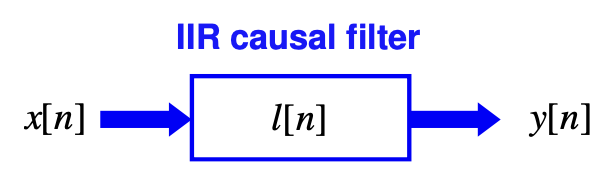
\includegraphics[width=0.5\linewidth]{Image/pdf 2/1.IIR .png}
    \label{fig:placeholder}
\end{figure}
\begin{itemize}
    \item \(x[n]\) is a white random process, so \(R_X[m]=\sigma^2_X\delta[m]\).
    \item The output \(y[n]\) can be expressed as : \(y[n]=\sum_{k=0}^{+\infty}l[k]x[n-k]\).
    \item Then, the cross-correlation function between \(x[n]\)a and \(y[n]\) is:
    
\[
R_{XY}[m] \triangleq E\{x[n]y[n+m]\} = E\left\{ x[n] \sum_{k=0}^{+\infty} l[k] x[n+m-k] \right\}
\]

\[
= \sum_{k=0}^{+\infty} l[k] E \{ x[n] x[n+m-k] \}
= \sum_{k=0}^{+\infty} l[k] R_X[m-k]
= \sigma_X^2 l[m]
\]
\item Since \(l[n]\) is casual, we have: \(R_{XY}[m]\neq0\) only if \(m\geq 0\) \(\Rightarrow\) \(R_{XY}[m]\neq R_{XY}[-m]\)
\item In particular, let \(x[n_0]\) and \(y[n_1]\) be two samples from the input and from the output signals, respectively.
\item If \(n_0<n_1\), i.e. \(m=n_1-n_0>0\), due to the filter memory, the input at \(n_0\) affects the output at \(n_1\), so \(x[n_0]\) and \(y[n_1]\) are NOT correlated.

\begin{figure}[H]
    \centering
    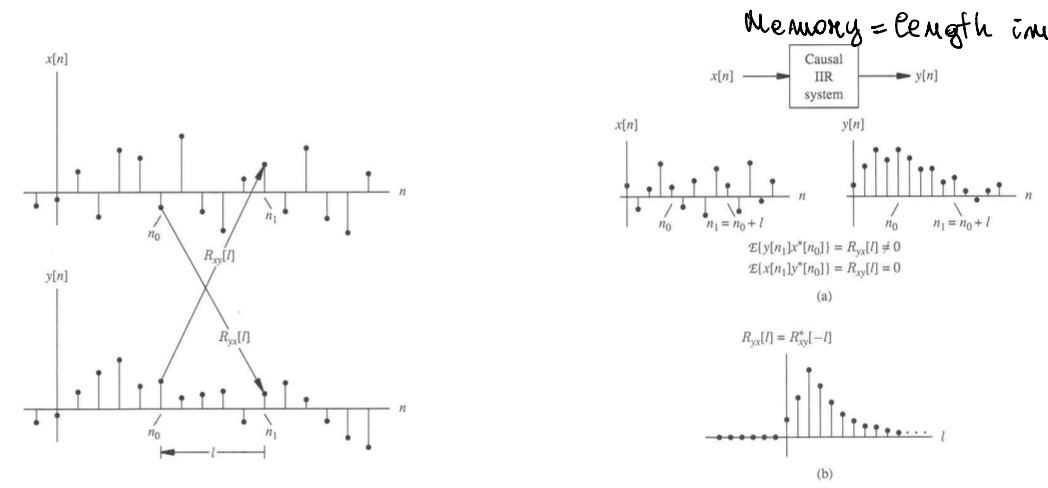
\includegraphics[width=0.75\linewidth]{Image/pdf 2/2.Example.png}

    \label{fig:placeholder}
\end{figure}
\end{itemize}

\subsection{Power Spectral Density(PSD)}
\noindent There are two possible definitions of the \textbf{PSD} of a w.s.s discrete-time random process:
\textbf{Definition 1:}
\[
S_X(e^{j 2\pi f}) \triangleq \lim_{N \to \infty} \frac{1}{N} E\left\{ \left| X_N(e^{j 2\pi f}) \right|^2 \right\}
\]

\[
\text{dove} \quad X_N(e^{j 2\pi f}) \triangleq DTFT\{x[n]\} = \sum_{n=0}^{N-1} x[n] e^{-j 2\pi f n}
\]
\\


\noindent \textbf{Definition 2:}

\[
S_X(e^{j2\pi f}) \triangleq DTFT\{R_X[m]\} = \sum_{m=-\infty}^{\infty} R_X[m] e^{-j2\pi f m}
\]

\[
\text{dove} \quad R_X[m] \triangleq E\left\{ x[n] x^*[n+m] \right\} = R_X^*[-m]
\]

\noindent The second definition of the PSD is also known as the \textbf{Einstein-Wiener-Khintchine Theorem:}
\[
S_X\left(e^{j2\pi f}\right)\triangleq\sum_{m=-\infty}^{+\infty}R_X[m]e^{-j2\pi fm},\hspace{0.25em}|f|\leq1/2
\]
\noindent Note that the PSD is \textit{periodic} with period equal to 1.\\
\noindent The inverse relation is given by:
\[
R_X[m]=\int_{-1/2}^{1/2}S_X(e^{j2\pi f})e^{j2\pi fm}df
\]
\noindent The term PSD refer to:
\[
P_X\triangleq E\{|x[n]^2|\}=R_X[0]=\int_{-1/2}^{1/2}S_X(e^{j2\pi f})df
\]
Let \(x[n]\) be a \underline{real} discrete-time random process, then its PSD satisfies two fundamental properties:
\begin{enumerate}
    \item The PSD is a \textit{real} and \textit{even} function of \(f\):
    \[
S_X(e^{j 2\pi f}) \in \mathbb{R}, \qquad S_X(e^{j 2\pi f}) = S_X(e^{-j 2\pi f}), \qquad |f| \leq 1/2
\]
   \item The PSD is non-negative:
   \[
   S_X(e^{j2\pi f})\geq0, |f|\le1/2
   \]

\end{enumerate}
\subsubsection{The link between ACF and the PSD}
\begin{figure}[H]
    \centering
    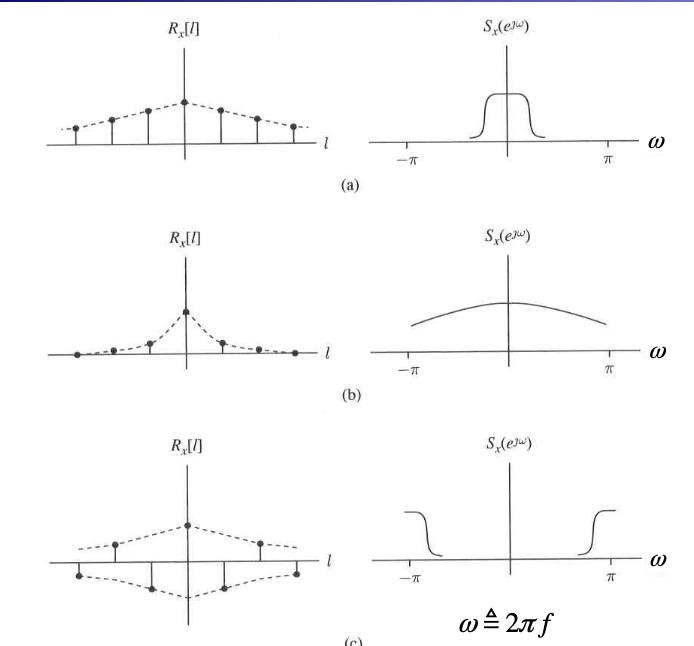
\includegraphics[width=0.35\linewidth]{Image/pdf 2/3.ACF_PSD.png}
    
    \label{fig:placeholder}
\end{figure}

\begin{itemize}
    \item When the ACF is broad, indicating small changes between samples of \(x[n]\), the PSD is narrow, i.e. \(x[n]\) has only low-frequency components.
    \item When the ACF is narrow, indicating low correlation between samples that are not too far, the PSD is broad, i.e. \(x[n]\) can have high-frequency components which allows it to change significantly (and irregularly) between successive samples.
    \item When the ACF shows rapidly varying characteristic, corresponding to negative correlation, the PSD contains \textit{only} high frequencies (i.e. close to \(1/2\))
\end{itemize}
\subsubsection{The PSD of a white discrete-time random process}
\begin{itemize}
    \item As previously, discussed, any discrete-time zero-mean random process whose samples are uncorrelated is called a \textbf{discrete-time white process}.
    \item Consequently, the ACF of a w.s.s discrete-time random process is:
    \[
    R_W[m]=\sigma^2_W\delta[m]
    \]
    \item Then, the PSD is given by:
    \[
    S_W(e^{j2\pi f})=\sigma_W^2\sum_{m=-\infty}^{+\infty}\delta[m]e^{-j2\pi f m}=\sigma_W^2
    \]
    \item Then PSD is constant over all the frequency band, and this fact justifies the name "white process".
    \item Unlike a continous-time white process, a discrete-time white process has finite power equal to:
    \[
    R_W[0]=\int_{-1/2}^{1/2}S_W(e^{j2\pi f})df=\int_{-1/2}^{1/2}\sigma_W^2df=\sigma_W^2
    \]
    \item In the most general case, the PSD can be written in the form:
    \[
S_X(e^{j2\pi f}) = S_X^c(e^{j2\pi f}) + 2\pi \sum_{i=1}^L P_i \, \delta\left( e^{j2\pi f} - e^{j2\pi f_i} \right)
\]
    \item The first term represents the continuous part of the spectrum, the second term is the discrete part, i.e. the Dirac's delta functions present in the spectrum.
    \item The Dirac's delta functions arise from \textit{periodic} or \textit{almost periodic} components of the discrete random process. The continuos part in the PSD is due to the aperiodic(or transient) components in the data.

\end{itemize}
NOTE: If you have \(s[n]=\cos(2\pi F_0n+\theta_0)\):
\begin{itemize}
    \item If \(F_0=K/N\) is a ratio between two integers, then \(s[n]\) is periodic.
    \item If \(F_0\) is not a rational number, then \(s[n]\) is said to be quasi-periodic.
\end{itemize}

\subsubsection{EXAMPLE: cosinusoidal process in Additive white Gaussian Noise(AWGN)}
\[
x[n]=s[n]+w[n]=A\cos(2\pi F_0n+\theta_0)+w[n],\hspace{0.5em}0\leq F_0\leq\frac{1}{2}
\]
The amplitude A can be modelled as a Rayleigh r.v., the phase \(\theta_0\) is typically modelled as a r.v. uniformly distributed in \([-\pi,\pi)\), both are independent of \(w[n]\).
\[
A\in\mathcal{R}(\sigma^2_A) \hspace{2em} \theta_0\in(-\pi,\pi)\hspace{2em}\text{A and \(\theta_0\) independent}
\]
\[
f_A(a)=\frac{a}{\sigma_A^2}e^{-\frac{a^2}{2\sigma_A^2}}u(a),\hspace{0.5em}E\{A^2\}=2\sigma^2_A
\]
Autocorrelation function(ACF):
\[
R_X[m] = E\left\{ x[n]x[n+m] \right\}
= E\left\{ \left( s[n] + w[n] \right) \left( s[n+m] + w[n+m] \right) \right\}
\]\[
= R_S[m] + R_{SW}[m] + R_{WS}[m] + R_W[m]
= R_S[m] + R_W[m]
\]
Autocorrelation function of the cosinusoidal process:
\[
R_S[m] = E\{s[n]s[n+m]\} 
= E\{A^2\} E\{\cos(2\pi F_0 n + \theta_0)\cos(2\pi F_0 (n+m) + \theta_0)\}
\]
\[
= \frac{E\{A^2\}}{2} E\{\cos(2\pi F_0 m) + \cos(2\pi F_0 (2n+m) + 2\theta_0)\}
= \sigma_A^2 \cos(2\pi F_0 m)
\]
where the last equality follows from the Werner formula and from the fact that:
\[
E\left\{ \cos\left(2\pi F_0(2n+m)+2\theta_0\right) \right\}
= \frac{1}{2\pi} \int_{-\pi}^{\pi} \cos\left(2\pi F_0 (2n+m) + 2\theta_0 \right) d\theta_0 = 0, \quad \forall n \in \mathbb{Z}
\]
Autocorrelation function of the AWGN:
\[
R_W[m]=\sigma_W^2[m]
\]
Finally, the autocorrelation function of \(x[n]\) can be expressed as:
\[
R_X[m]=R_S[m]+R_W[m]=\sigma_A^2\cos(2\pi F_0m)+\sigma_W^2\delta[m]
\]
The mean value of \(x[n]\) is:
\[
E\{x[n]\} = E\{s[n]\} + E\{w[n]\}
= E\left\{A\cos\left(2\pi F_0 n + \theta_0\right)\right\}
= E\{A\} E\left\{\cos\left(2\pi F_0 n + \theta_0\right)\right\} = 0
\]
where the last equality follows from the Werner formula and from the fact that:
\[
E\left\{ \cos\left(2\pi F_0(2n+m)+2\theta_0\right) \right\}
= \frac{1}{2\pi} \int_{-\pi}^{\pi} \cos\left(2\pi F_0 (2n+m) + 2\theta_0 \right) d\theta_0 = 0, \quad \forall n \in \mathbb{Z}
\]
Since the mean is constant and the ACF is a function of only the lag \(m\), the process \(x[n]\) is a wide sense stationary (w.s.s) process. Hence, we can calculate the Power Spectral Density.\\

The \textbf{PSD} is given by the FT of the ACF:
\[
S_X(e^{j2\pi f}) \triangleq \sum_{m=-\infty}^{+\infty} R_X[m] e^{-j2\pi f m}
= \mathcal{FT}\left\{ \sigma_A^2 \cos(2\pi F_0 m) + \sigma_w^2 \delta[m] \right\}
\]
\[
= \sigma_A^2 \mathcal{FT} \left\{ \cos(2\pi F_0 m) \right\} + \sigma_w^2 \mathcal{FT} \left\{ \delta[m] \right\}
= 2\pi \cdot \frac{\sigma_A^2}{2} \left[ \delta\left( e^{j2\pi f} - e^{j2\pi F_0} \right) + \delta\left( e^{j2\pi f} - e^{-j2\pi F_0} \right) \right] + \sigma_w^2
\]
The \textbf{statistical power} of the cosinusoidal process \(s[n]\):
\[
P_S = E\{s^2[n]\} = R_S[0] = \frac{E\{A^2\}}{2} = \sigma_A^2
\]

\[
P_S = \int_{-1/2}^{1/2} S_S(e^{j2\pi f}) \, df
\]

\[
= \int_{-1/2}^{1/2} 2\pi \cdot \frac{\sigma_A^2}{2} 
\left[ \delta \left( e^{j2\pi f} - e^{j2\pi F_0} \right)
+ \delta \left( e^{j2\pi f} - e^{-j2\pi F_0} \right) \right]
\, df
\]

\[
= \frac{\sigma_A^2}{2} \int_{-1/2}^{1/2} 2\pi \cdot \delta(e^{j2\pi f} - e^{j2\pi F_0}) \, df
+ \frac{\sigma_A^2}{2} \int_{-1/2}^{1/2} 2\pi \cdot \delta(e^{j2\pi f} - e^{-j2\pi F_0}) \, df
\]

\[
= \frac{\sigma_A^2}{2} \int_{-\pi}^{\pi} \delta(e^{j\omega} - e^{j2\pi F_0}) \, d\omega
+ \frac{\sigma_A^2}{2} \int_{-\pi}^{\pi} \delta(e^{j\omega} - e^{-j2\pi F_0}) \, d\omega
\]

\[
= \frac{\sigma_A^2}{2} + \frac{\sigma_A^2}{2} = \sigma_A^2
\]
\subsubsection{Costant signal(periodic) in AWGN(aperiodic)}
\[
x[n]=A+v[n]
\]
\begin{itemize}
    \item \(v[n]\) is a stationary white process with variance \(\sigma^2\)
    \item \(A\sim\mathcal{N}(\eta_A,\sigma_A^2)\) is independent of \(v[n]\) \underline{a periodic component at zero frequency}.
    \item The mean of process is: \(\eta_X=\eta_A\)
    \item The ACF: \(R_X[m]=\sigma_A^2+\eta_A^2+\sigma^2\delta[m]\)
    \item The PSD is given by: \[
S_X\left(e^{j2\pi f}\right)
= \mathcal{FT}\{ R_X[m] \}
= \mathcal{FT}\{ \sigma_A^2 + \eta_A^2 \} + \mathcal{FT}\{ \sigma^2 \delta[m] \}
\]
\[
= 2\pi \cdot (\sigma_A^2 + \eta_A^2)\, \delta\left(e^{j2\pi f} - 1\right) + \sigma^2
\]
\end{itemize}
The idea is the following: it's impossible to discriminate between:
\begin{itemize}
    \item A random process \(x[n]\) with a non-zero mean value \(\eta_X\), that has a Dirac's delta function at \(f=0\) of area \(\eta_X^2\) in the PSD.
    \item A random process \(x[n]\) with a zero mean random constant component has a Dirac's delta function at \(f=0\) of area \(var\{A\}\) in the PSD.
\end{itemize}
\subsection{Complex Power Spectral Density}
\begin{itemize}
    \item The use of the \textbf{z-transform} in the analysis of stationary discrete-time random processes is of fundamental importance.
    \item A quantity related to the second order moments of a stationary discrete-time random process in the domain of the z-transform is the \textbf{complex PSD}:
    \[
S_X(z) \triangleq ZT\left\{ R_X[m] \right\}
= \sum_{m=-\infty}^{+\infty} R_X[m]z^{-m},
\quad z \in \text{ROC} \subseteq \mathbb{C}
\]
   \item \textbf{ROC = Region of convergence}, i.e. those values of z fro which the sum above converges to a finite value.
   \item The ROC of a complex PSD is always an annular region, i.e. of the form:
   \[
   ROC\equiv\{z|\rho<|z|<1/\rho|\}, \hspace{0.5em}\text{with }0<\rho<1
   \]
   \item The PSD introduced before can be regarded as a special case of the CPSD when the latter is evaluated on the unit circle(the unit circle belongs to the ROC):
   
\begin{figure}[H]
    \centering
    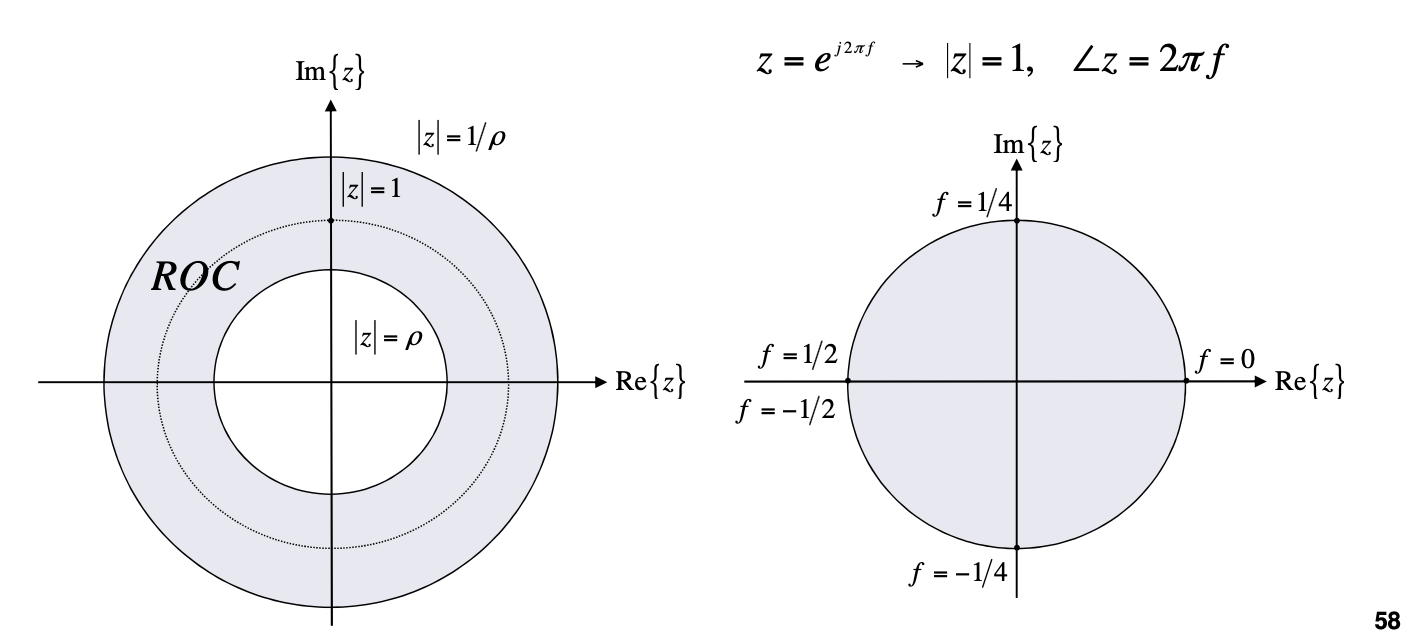
\includegraphics[width=0.75\linewidth]{Image/pdf 2/4.ROC.png}
    \label{fig:placeholder}
\end{figure}
    \item The inverse formula is:
    \[
    R_X[m]=\frac{1}{j2\pi}\oint_{\partial C}S_X(z)z^{m-1}dz
    \]
    When the contour of the integration region \(C\), i.e. \(\partial C\), is taken to be counterclockwise and in the convergence region of the z-transform.
    \item From the property of symmetry of the ACF, \(R_X[-m]=R_X^*[m]\),we have that:
    
\[
S_X(z) = \sum_{m=-\infty}^{+\infty} R_X[m] z^{-m}
= \sum_{m=-\infty}^{+\infty} R_X[-m] z^m
= \left( \sum_{m=-\infty}^{+\infty} R_X[m] \left( \frac{1}{z^*} \right)^{-m} \right)^*
= S_X^*\left(\frac{1}{z^*}\right)
\]
   \item For \underline{real-valued} random processes, i.e. for real ACFs, we have:
   \[
S_X(z) = S_X^*\left(\frac{1}{z^*}\right) = S_X\left(\frac{1}{z}\right) = S_X\left(z^{-1}\right)
\]
   \item As for the PSD, the complex PSD can be written in the form:
   \[
S_X(z) = S_X^c(z) + 2\pi \sum_{i=1}^{L} P_i \delta \left(z - e^{j2\pi f_i} \right)
\]
\end{itemize}
As for the PSD, the complex PSD can be written in the form:

\noindent The first term represents the continuos part of the spectrum, the second term is the discrete part, i.e. the Dirac's delta functions present in the spectrum.\\
The Dirac's delta functions arise from \textit{periodic} or \textit{almost periodic} components of the random process. The continuous part is due to the \textit{aperiodic} components of the random process.\\
\textbf{IMPORTANT}: Note that, due to mathematical problems related to the Dirac's delta function, the direct and the inverse formulas that link the complex PSD and the ACF are valid only for the continuous part of the complex PSD.

\subsubsection{Poles and zeros}

The continuous part of the complex PSD can be usually expressed as the ratio of two polynomials in z.
\begin{itemize}
    \item Due to the following relations for \textit{complex-valued} and \textit{real-valued} random processes:
    \[
    S_X(z)=S^*_X(1/z^*)\qquad S_X(z)=S_X(z^{-1})
    \]
    The polynomials at the numerators and at the denomiantor have to be factorized as:
    \[
\left( 1 - z_0 z^{-1} \right)
\;\rightarrow\;
\left( 1 - z_0 z^{*} \right)^{*}
= \left( 1 - z_0^{*} z \right)
\;\Rightarrow\;
\left( 1 - z_0 z^{-1} \right)
\left( 1 - z_0^{*} z \right)
\]
    \item This implies that for every pole (and zero) that occurs at
    \[
    z_0=|z_0|e^{j\phi_0}
    \]
    there is a corresponding pole (and zero) at
    \[
\frac{1}{z_0^{*}}
= \left( \frac{1}{|z_0|} e^{-j\phi_0} \right)^{*}
= \frac{1}{|z_0|} e^{j\phi_0}
\]
    \item Hence, poles and zeros of the CPSD occur at conjugate reciprocal positions.
    \item For \underline{real-valued} processes the CPSD can be expressed in terms of real polynomials in z, as a consequence the roots must occur in conjugate pairs.
    \item This implies that for real-valued random processes, poles and the zeros of the complex PSD occur in \underline{group of four} at locations:
    \[
    z_0 \qquad 1/z_0^*\qquad z_0^* \qquad1/z_0
    \]
    \item Roots on real axis occur in pair at locations: \(z_0,1/z_0\)
    \item When zeros occur on the unit circle, they must occur in even multiplicities.
    \item Poles on the unit circle are not allowed to exist; they could eventually contribute to the discrete part of the complex PSD.
    \item A pole(zero) at the origin implies a pole(zero) at \(\infty\)
\end{itemize}
\begin{figure}[H]
    \centering
    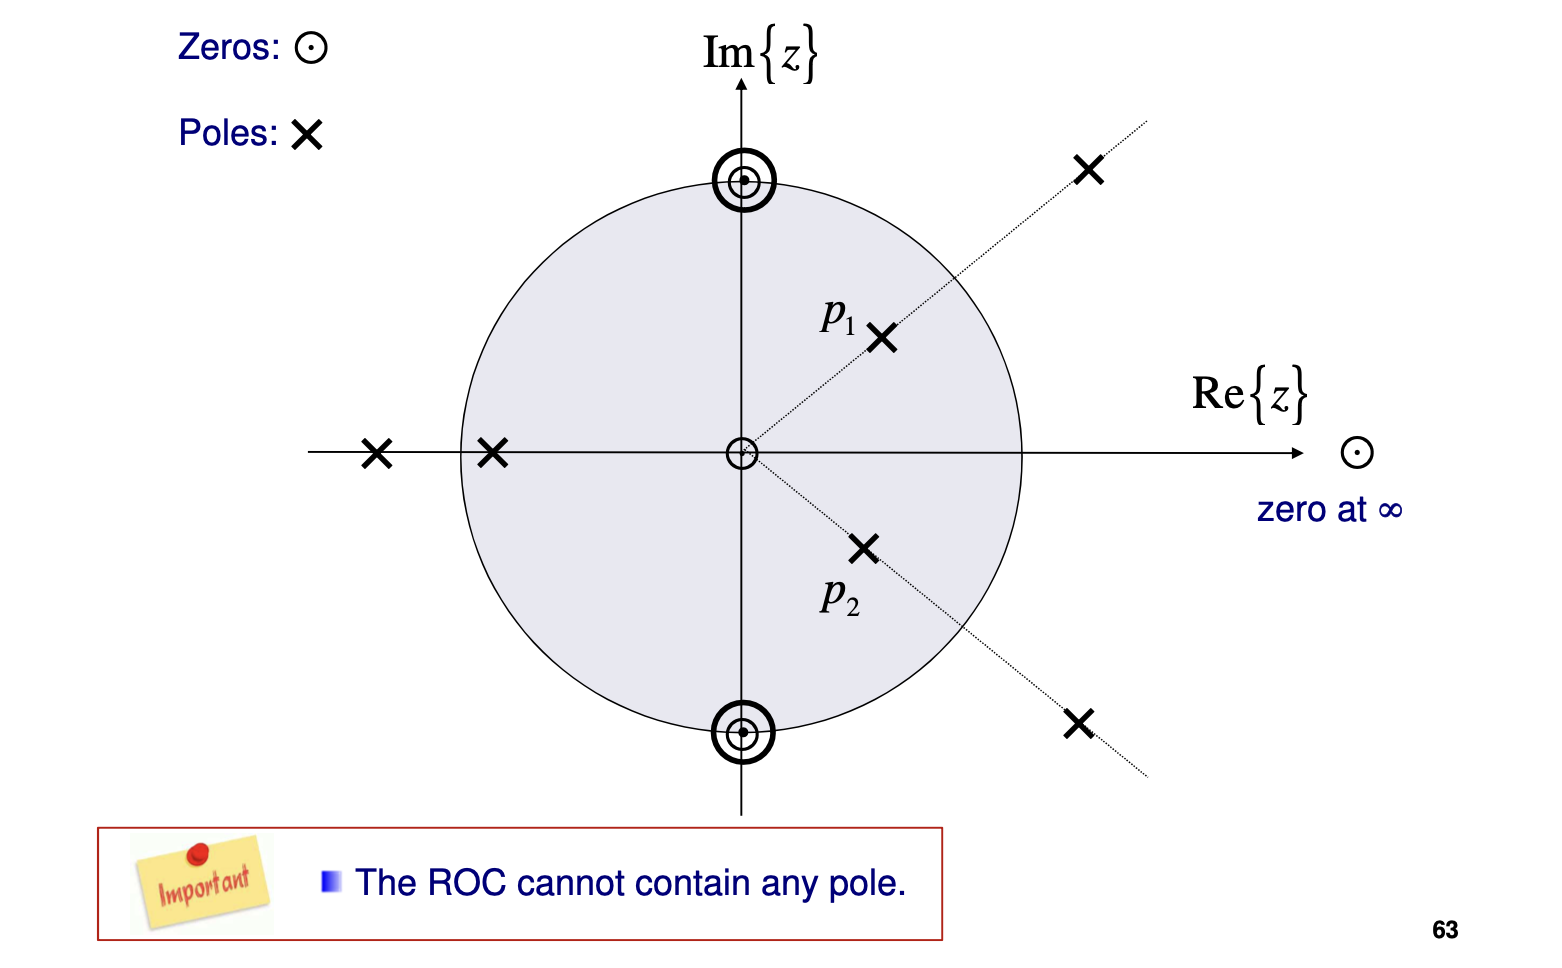
\includegraphics[width=0.75\linewidth]{Image/pdf 2/5.pole_zero.png}
    \label{fig:placeholder}
\end{figure}
\subsubsection{Region of convergence}
\begin{itemize}
     \item The symmetry property of the complex PSD of real-valued processes, i.e.
\[
S_X(z)=S_X(z^{-1}) \qquad(*)
\]
     has specific implications in the shape of the region of convergence.
     \item In particular, if \(S_X(z)\) converges only in the region \(|z|<\rho\) where \(\rho\) is a positive real number, because of property(*), \(S_X(z)\) should also converge for z such that \(|z^{-1}|>\rho\) i.e. \(|z|<1/\rho\)
     \item Then, the complex PSD always converges on an annular region of the form:
     \[
     \rho<|z|<1/\rho, \qquad o<\rho<1
     \]
     \item \(\rho\) must be strictly less then 1, otherwise the convergence region is an empty set.
     
\end{itemize}
\noindent\textbf{IMPORTANT}: The unitary circle belongs to the convergence region.
\subsection{Linear time-invariant systems}
A linear time-invariant (LTI) system can be characterized by its \textit{impulse response}, say \(l[n]\).\\
The impulese response is defined as the output of the LTI system when the input is the Kronecker delta function with unit amplitude.\\
The system input and output are related by the linear convolution operator:
\[
x[n] = w[n] \otimes l[n] = \sum_{k=-\infty}^{+\infty} l[k]\,w[n-k] = \sum_{k=-\infty}^{+\infty} w[k]\,l[n-k]
\]

\noindent Along with the \textit{impulse response} \(l[n]\) , an LTI system can be equivalently characterized by the \textit{frequency response} and by \textit{transfer function}.\\
\begin{itemize}
    \item The \textbf{transfer function} is defined as the \(Z-\)transform of \(l[n]\):
\[
L(z)=Z\{l[n]\}=\sum_{n=-\infty}^{+\infty}l[n]z^{-n}
\]
    \item The \textbf{frequency response} is defined as the Fourier Transform of \(l[n]\):
    \[
    L(e^{j2\pi f})=FT\{l[n]\}=\sum_{n=-\infty}^{+\infty}l[n]e^{-j2\pi f n}=L(z)\Big|_{z=e^{j2\pi f}}
    \]
    \item We are interested in the functional relations that link the first and second order moments of a random process at the input of the LTI system with those at the output.
    \item The mean value functions of the input and output random processes are related by the following expression:
    \[
\eta_X[n] = E\{x[n]\} = E\{w[n] \otimes l[n]\} = E\{w[n]\} \otimes l[n] = \eta_W[n] \otimes l[n]
\]
    \item If the input is a w.s.s. random process, then:
    \[
\eta_X[n] = E\{x[n]\} = E\{w[n] \otimes l[n]\} = E\{w[n]\} \otimes l[n] = \eta_W[n] \otimes l[n]
\]
    \item If \(w[n]\) is a w.s.s. random process, then the output \(x[n]\) is a w.s.s. as well. Moreover, \(w[n]\) and \(x[n]\) are \textit{jointly wide-sense stationary}.
    \item The ACF of the output of an LTI system can be expressed:
    \[
\begin{aligned}
R_X[m] &= E\{x[n] x[n+m]\} = E\left\{ \sum_{k=-\infty}^{+\infty} l[k] w[n-k] x[n+m] \right\} \\
&= \sum_{k=-\infty}^{+\infty} l[k] E\{ w[n-k] x[n+m] \}
= \sum_{k=-\infty}^{+\infty} l[k] R_{WX}[m+k] \\
&= l[m] \otimes R_{WX}[-m]
\end{aligned}
\]
where \(R_{WX}[m]\) is the cross-correlation function between the input and the output.
\item The cross-correlation function \(R_{WX}[m]\) can be explicitly evaluated as:
\[
\begin{aligned}
R_{WX}[m] &= E\{ w[n] x[n+m] \} = E\left\{ w[n] \sum_{k=-\infty}^{+\infty} l[k] w[n+m-k] \right\} \\
&= \sum_{k=-\infty}^{+\infty} l[k] E\{ w[n] w[n+m-k] \}
= \sum_{k=-\infty}^{+\infty} l[k] R_W[m-k] \\
&= l[m] \otimes R_W[m]
\end{aligned}
\]
\item Finally, the ACF of the output of a LTI system is:
\[
R_X[m] = l[m] \otimes R_{WX}[-m] = l[m] \otimes l[-m] \otimes R_W[-m] = l[m] \otimes l[-m] \otimes R_W[m]
\]
\[
R_X[m] = l[m] \otimes l[-m] \otimes R_W[m]
\]
\item By exploiting the properties of the convolution operator and of the Fourier Transform, the relation between the PSDs of the input and output is:
\[
\begin{aligned}
S_X \left( e^{j2\pi f} \right) &= FT\{R_X[m]\} = FT\left\{ l[m] \otimes l[-m] \otimes R_W[m] \right\} \\
&= L\left(e^{j2\pi f}\right) L\left(e^{-j2\pi f}\right) S_W\left(e^{j2\pi f}\right) \\
&= L\left(e^{j2\pi f}\right) L^*\left(e^{j2\pi f}\right) S_W\left(e^{j2\pi f}\right) \\
&= \left|L\left(e^{j2\pi f}\right)\right|^2 S_W\left(e^{j2\pi f}\right)
\end{aligned}
\]
\item Similarly, using the properties of the Z-transform, we can derive the input-output relation for the complex PSD:
\[
\begin{aligned}
S_X(z) &= ZT\{R_X[m]\} = ZT\{l[m] \otimes l[-m] \otimes R_W[m]\} \\
&= L(z) L(1/z) S_W(z)
\end{aligned}
\]
\item If the input process \(w[n]\) is a white process, i.e.
\[
R_W[m]=\sigma_W^2\delta[m]\qquad S_W(e^{j2\pi f})=\sigma_W^2
\]
the previous simplify to :
\[
R_X[m] = R_W[m] \otimes l[m] \otimes l[-m] = \sigma_W^2 l[m] \otimes l[-m]
\]

\[
S_X\left(e^{j2\pi f}\right) = S_W\left(e^{j2\pi f}\right) \left|L\left(e^{j2\pi f}\right)\right|^2 = \sigma_W^2 \left|L\left(e^{j2\pi f}\right)\right|^2
\]

\[
S_X(z) = L(z) L(1/z) S_W(z) = \sigma_W^2 L(z) L(1/z)
\]

\end{itemize}
\subsubsection{The autoregressive process of order 1: AR(1)}
\begin{itemize}
    \item The input process \(w[n]\) is a white process, i.e.
    \[
    R_W[m]=\sigma_W^2\delta[m]\qquad S_W(e^{j2\pi f})=\sigma_W^2
    \]
    \item An \textbf{AR(1) process} is characterized by the following linear difference equation:
    \[
    x[n]=\rho x[n-1]+w[n],\qquad |\rho|<1
    \]
    \item An \textbf{AR(1) process}, also called \textbf{Markov process}, can be thought as the output of an IIR(1) LTI syste, with a suitable impulsive response driven by a white process.
    \item The \textbf{impulse response} \(l[n]\) of the IIR(1) filter that generates an AR(1) process can be evaluated by solving the relevant linear difference equation with a Kronecker delta as input sequence:    \[
x[n] = \rho x[n-1] + w[n]
\]
\[
\Downarrow
\]
\[
l[n] = \rho l[n-1] + \delta[n], \quad \text{with} \ l[-1]=0\ \text{and}\ |\rho| < 1
\]
\[
\Downarrow
\]
\[
\left\{
\begin{array}{l}
l[0] = \rho l[-1] + \delta[0] = 1 \\
l[1] = \rho l[0] + \delta[1] = \rho \\
l[2] = \rho l[1] + \delta[2] = \rho^2 \\
\vdots \\
l[n] = \rho l[n-1] + \delta[n] = \rho^n
\end{array}
\right.
\]
    \item Then, finally : \(l[n]=\rho^nu[n],\qquad|\rho|<1\)
    \item In order to evaluate the \textbf{frequency response},we rely on the Z-transform of both sides of the linear difference equation characterizing the AR(1) process:
\[
x[n] = \rho x[n-1] + w[n], \quad |\rho| < 1
\]
\[
\Downarrow
\]
\[
X(z) = \rho z^{-1} X(z) + W(z), \quad |\rho| < 1
\]
\[
\Downarrow
\]
\[
\left(1 - \rho z^{-1}\right) X(z) = W(z), \quad |\rho| < 1
\]
\[
\Downarrow
\]
\[
L(z) = \frac{X(z)}{W(z)} = \frac{1}{1 - \rho z^{-1}} = \frac{z}{z-\rho}, \quad |\rho| < 1
\]
    \item Then: \[L(e^{j2\pi f})=L(z)\Big|_{z=e^{j2\pi f}}=\frac{1}{1-\rho e^{-j2\pi f}},\qquad|\rho|<1\]
    \item Alternatively, the \textbf{frequency response} can be derived as the Fourier Transform (FT) of the impulse response \(l[n]\):
    \[
L\left(e^{j2\pi f}\right) = FT\{l[n]\} = \sum_{n=-\infty}^{+\infty} l[n] e^{-j2\pi f n} = \sum_{n=-\infty}^{+\infty} \rho^n u[n] e^{-j2\pi f n}
\]

\[
= \sum_{n=0}^{+\infty} \rho^n e^{-j2\pi f n} = \sum_{n=0}^{+\infty} \left(\rho e^{-j2\pi f}\right)^n
\]

\[
= \frac{1}{1 - \rho e^{-j2\pi f}} \qquad \text{iff} \quad \left|\rho e^{j2\pi f}\right| = |\rho| < 1
\]
\item Parameter \(\rho\) represents the \textbf{one-lag correlation coefficient} of the process:
\begin{figure}[H]
    \centering
    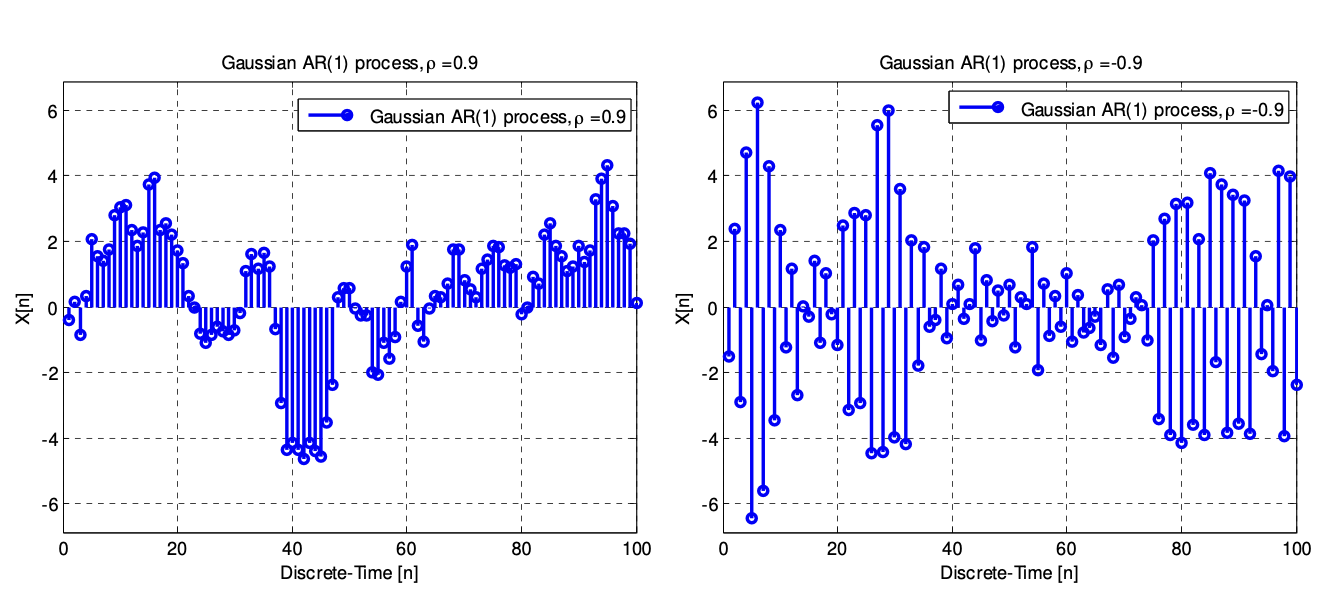
\includegraphics[width=0.75\linewidth]{Image/pdf 2/6.Lag_rho.png}
    \label{fig:placeholder}
\end{figure}
\[
S_X\left(e^{j2\pi f}\right) = \sigma_W^2 \left|L\left(e^{j2\pi f}\right)\right|^2 = \sigma_W^2 \left| \frac{1}{1 - \rho e^{-j2\pi f}} \right|^2 = \frac{\sigma_W^2}{1 + \rho^2 - 2\rho \cos(2\pi f)}
\]
\begin{figure}[H]
    \centering
    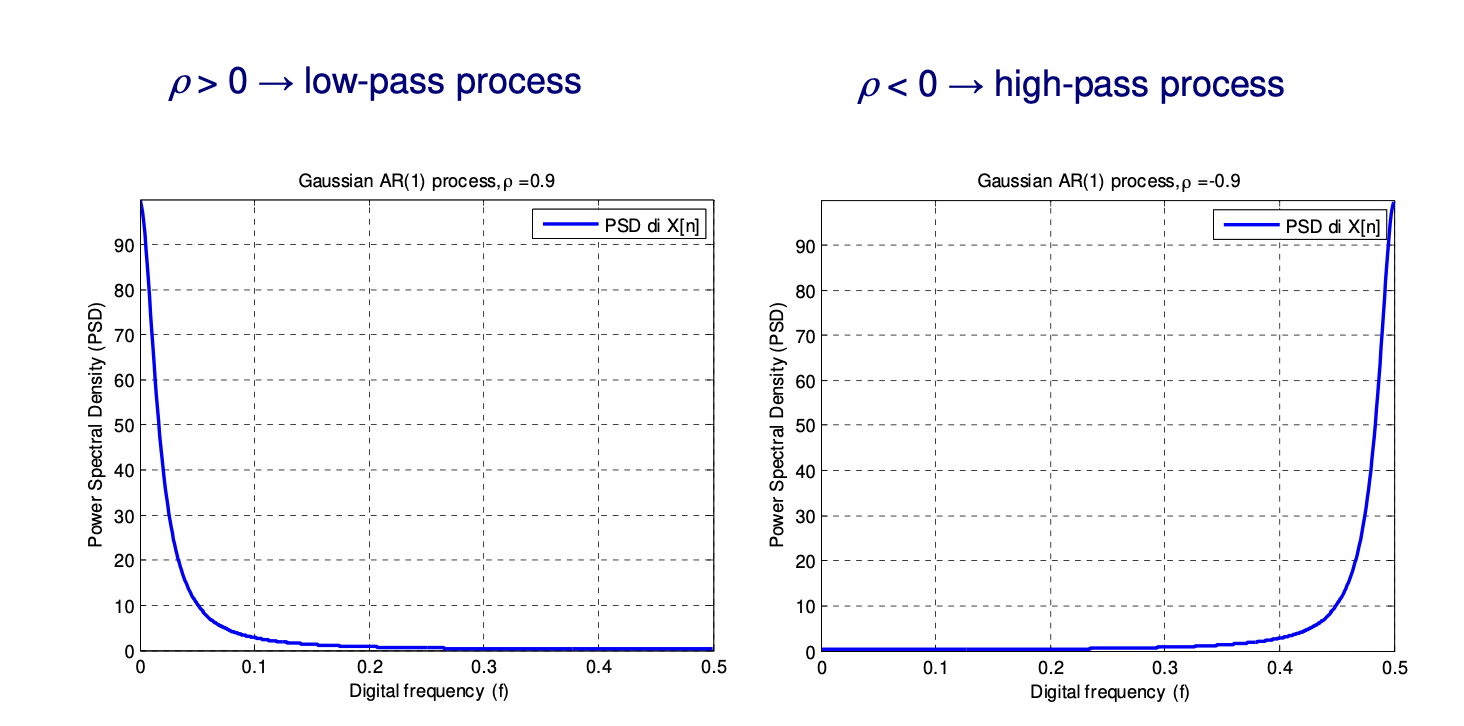
\includegraphics[width=0.75\linewidth]{Image/pdf 2/7.LP_HP.png}
    \label{fig:placeholder}
\end{figure}
\item With ar AR(1) model we can obtain/represent only low-pass or high-pass processes, but not pass-band processes.
\item The bandwidth \(B\) of the process depends on how close the pole is to the unit circle: \(B\) gets lower when \(\rho\) gets closer to the unit circle.
\begin{figure}[H]
    \centering
    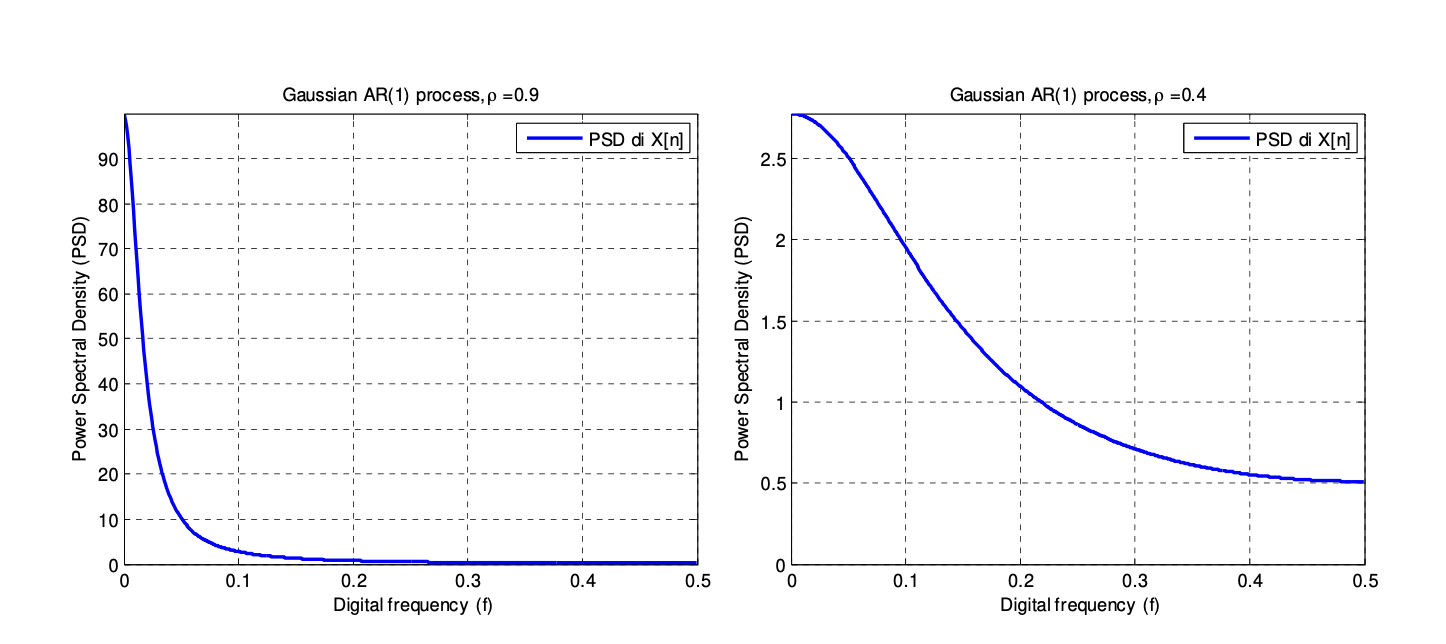
\includegraphics[width=0.75\linewidth]{Image/pdf 2/8.Bandwidth.png}
    \label{fig:placeholder}
\end{figure}
\item \textbf{Autocorrelation function (ACF)} of an AR(1) process:
\[
R_X[m] = E\{x[n]x[n+m]\} 
      = E\left\{ x[n] \left( \rho x[n+m-1] + w[n+m] \right) \right\} =\]\[
      = E\{ \rho x[n]x[n+m-1] + x[n]w[n+m] \} 
      = \rho R_X[m-1], \quad |\rho|<1, \ m>0 \]\[
\text{in fact} \quad E\{x[n]w[n+m]\} = 0 \text{ if } m > 0
\]

\item \(x[n]w[n+m]\) is 0, since the output at time \(n\) cannot depend on the input at time \(n+m>n\), being the filter causal. Also we can say:
\[
R_X[m]=R_X[0]\rho^m, \qquad|\rho|<1 \text{ and } m>0
\]
\item To derive the "initial condition" \(R_X[0]\):
\[
\begin{aligned}
\sigma_X^2 &= R_X[0] = E\{x^2[n]\} = E\left\{ \left( \rho x[n-1] + w[n] \right)^2 \right\} \\
&= \rho^2 E\{x^2[n-1]\} + 2\rho E\{x[n-1] w[n]\} + E\{w^2[n]\} \\
&= \rho^2 \sigma_X^2 + \sigma_W^2
\end{aligned}
\]
\[
\sigma_X^2=\frac{\sigma_W^2}{1-\rho^2},\qquad|\rho|<1
\]
\item Taking into account that for real processes \(R_X[-m]=R_X[m]\), we finally have:
\[
R_X[m]=\frac{\sigma_W^2}{1-\rho^2}\rho^{|m|}, \qquad|\rho|<1
\]
\[
R_X[m] = \frac{\sigma_w^2}{1-\rho^2} \rho^{|m|}
\implies
\rho_X = \frac{\text{cov}\{X[n], X[n+1]\}}{\sqrt{\text{var}\{X[n]\} \text{var}\{X[n+1]\}}}
= \frac{R_X[1]}{R_X[0]} = \rho
\]
\item Hence, the parameter \(\rho\) is \textbf{one-lag correlation coefficient}.
\begin{figure}[H]
    \centering
    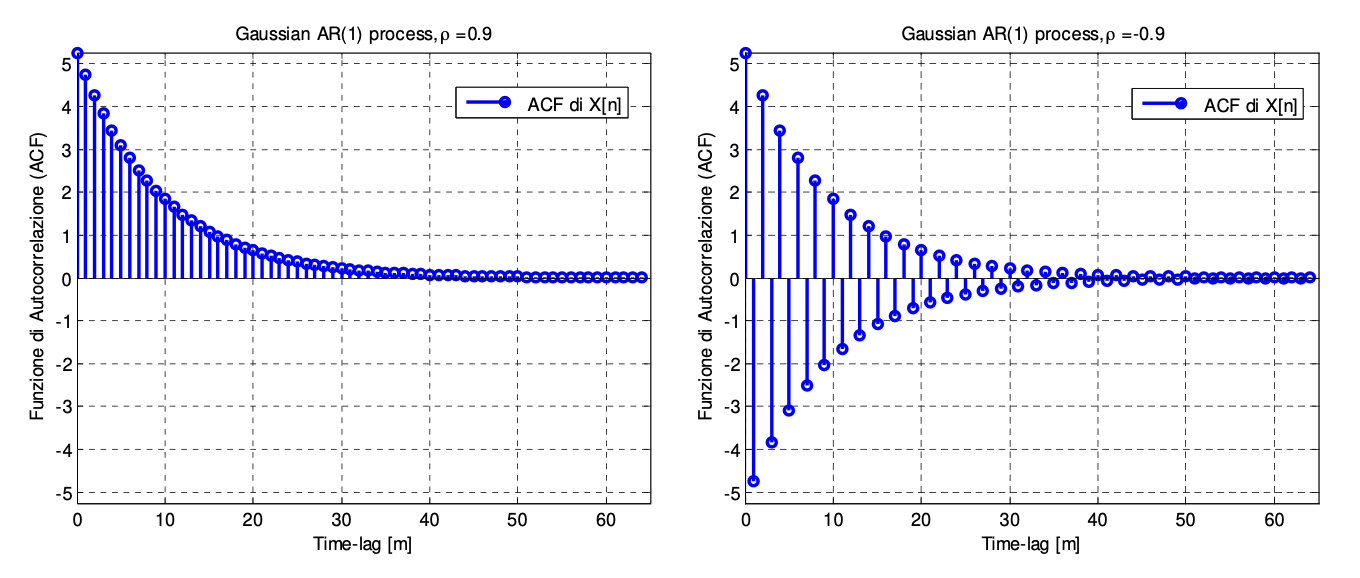
\includegraphics[width=0.75\linewidth]{Image/pdf 2/9.One_lag.png}
    \label{fig:placeholder}
\end{figure}
\item The duration of the ACF (\textbf{correlation time} or \textbf{coherence time}) is larger when \(|\rho|\) is closer to the unit circle.
\begin{figure}[H]
    \centering
    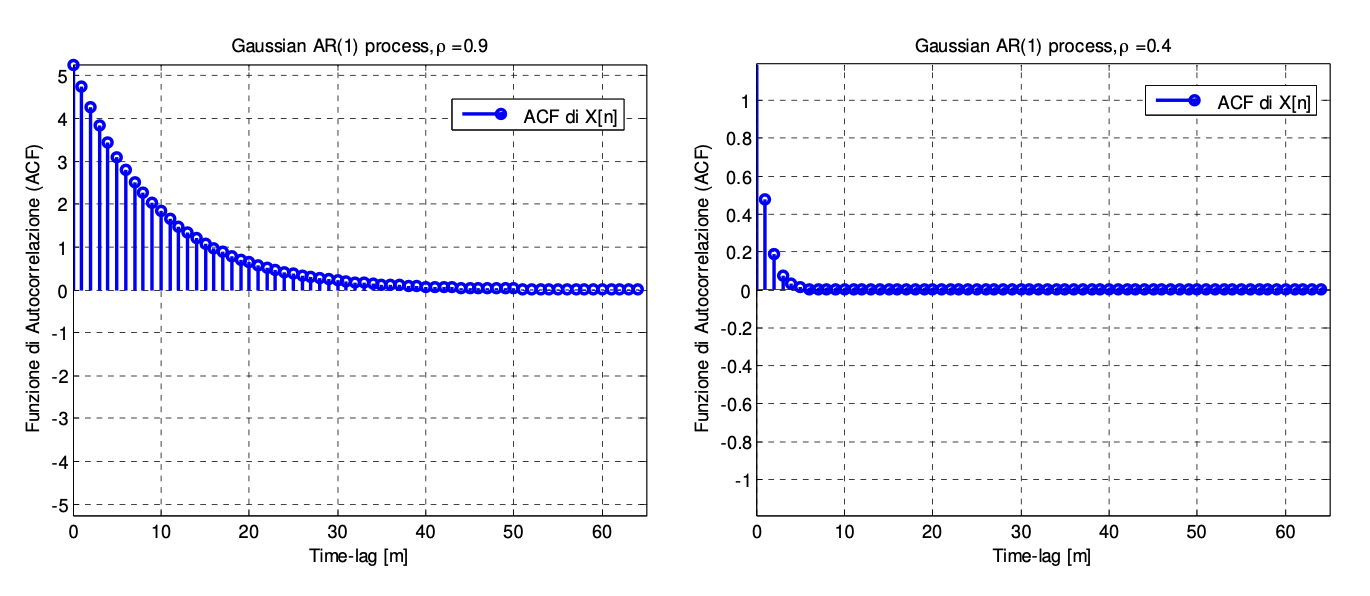
\includegraphics[width=0.75\linewidth]{Image/pdf 2/10.ACF_dur.png}
    \label{fig:placeholder}
\end{figure}
\end{itemize}
\subsubsection{Moving average process or order 1}
\begin{figure}[H]
    \centering
    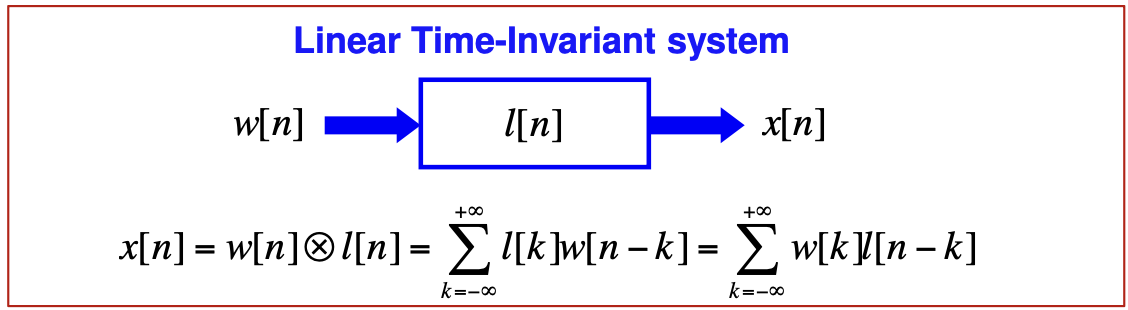
\includegraphics[width=0.75\linewidth]{Image/pdf 2/11.LTI_system.png}
    \label{fig:placeholder}
\end{figure}
\begin{itemize}
    \item The input process \(w[n]\) is a white process, i.e.
    \[
    R_W[m]=\sigma_W^2\delta[m]\qquad S_W(e^{j2\pi f})=\sigma_W^2
    \]
    \item An \textbf{MA(1) process} i characterized by the following linear difference equation:
    \[
    x[n]=w[n]+b_1w[n-1], \qquad|b_1|<1
    \]
    \item An \textbf{MA(1) process} can be thought as the output of an FIR(1) LTI system with a suitable impulsive response driven by a white process.
    \item Let us first derive the \textbf{impulse response} \(l[n]\) of the FIR(1) and its \textbf{frequency response}:
    \[
x[n] = w[n] + b_1 w[n-1], \quad |b_1| < 1
\]
\[
l[n] = \delta[n] + b_1 \delta[n-1] \implies
l[n] = 
\begin{cases}
1, & n = 0 \\
b_1, & n = 1 \\
0, & \text{otherwise}
\end{cases}
\]
\[
L(e^{j2\pi f}) = \mathcal{FT}\{l[n]\} = \sum_{n=-\infty}^{+\infty} \left(\delta[n] + b_1 \delta[n-1]\right) e^{-j2\pi f n}
= 1 + b_1 e^{-j2\pi f}
\]
\[
X(z) = W(z) + b_1 z^{-1} W(z) \implies
L(z) = \frac{X(z)}{W(z)} = 1 + b_1 z^{-1}
\]
\[
L(z) = 0 \implies z = -b_1 \implies \text{1 zero} \; z_1 = -b_1
\]
\item Let us now derive the \textbf{Autocorrelation function(ACF)}
\[
R_X[m] = E\{x[n]x[n+m]\}
\]
\[
= E\left\{ \left(w[n] + b_1 w[n-1]\right) \left(w[n+m] + b_1 w[n+m-1]\right) \right\}
\]
\[
= R_W[m] + b_1 R_W[m-1] + b_1 R_W[m+1] + b_1^2 R_W[m]
\]
\[
= (1 + b_1^2) \sigma_w^2 \delta[m] + b_1 \sigma_w^2 \delta[m-1] + b_1 \sigma_w^2 \delta[m+1]
\]

\[
R_X[m]=(1+b_1^2)\sigma_w^2\delta[m] + b_1\sigma_w^2\delta[m-1] + b_1\sigma_w^2\delta[m+1]
\]

\[
R_X[m]=\begin{cases}
(1+b_1^2)\sigma_w^2,    & m=0 \\
b_1\sigma_w^2,          & m=\pm1 \\
0,                      & \text{otherwise}
\end{cases}
\]
\item The power of the process and the one-lag correlation coefficient are given by:
\[
R_X[0] = \sigma_X^2 = (1 + b_1^2) \sigma_w^2,
\quad
\rho_X[1] = \frac{R_X[1]}{R_X[0]} = \frac{b_1}{1 + b_1^2}
\]
\item The \textbf{Power Spectral Density(PSD)} can be derived as the FT of the ACF:
\[
S_X(e^{j2\pi f}) = \mathcal{FT}\{R_X[m]\} = \sum_{m=-\infty}^{+\infty} R_X[m] e^{-j2\pi f m}
\]
\[
= \sum_{m=-\infty}^{+\infty} \left[ (1+b_1^2) \sigma_w^2 \delta[m] + b_1 \sigma_w^2 \delta[m-1] + b_1 \sigma_w^2 \delta[m+1] \right] e^{-j2\pi f m}
\]
\[
= (1+b_1^2)\sigma_w^2 + b_1\sigma_w^2 e^{-j2\pi f} + b_1\sigma_w^2 e^{j2\pi f}
\]
\[
= \sigma_w^2 \left(1+b_1^2+2b_1\cos(2\pi f)\right)
\]
\[
\textbf{CONDITION}
\]
\[
b_1<0\Rightarrow\text{hig-pass process,}\qquad b_1>0\Rightarrow\text{low-pass process}
\]
\item The PSD can also be obtained from the frequency response of the FIR(1) filter:
\[
S_X(e^{j2\pi f}) = \sigma_w^2 \left| L(e^{j2\pi f}) \right|^2 = \sigma_w^2 \left| 1 + b_1 e^{-j2\pi f} \right|^2
\]
\[
= \sigma_w^2 \left( 1 + b_1 e^{-j2\pi f} \right) \left( 1 + b_1 e^{j2\pi f} \right)
\]
\[
= \sigma_w^2 \left( 1 + b_1^2 + b_1 e^{-j2\pi f} + b_1 e^{j2\pi f} \right)
\]
\[
= \sigma_w^2 \left( 1 + b_1^2 + 2b_1 \cos(2\pi f) \right)
\]

\end{itemize}



\clearpage